\documentclass[12pt]{exam}

\usepackage{graphicx}
\graphicspath{ {./images/} }

\lhead{ECON 2010}
\chead{Practice}
\lfoot{11/27/2023}
\rhead{Fall 2023}

%\printanswers
 \noprintanswers

\begin{document}

\section{Practice Questions}

\begin{questions}

    \question Consider the following marginal tax schedule

\begin{table}[h]
        \centering
    \begin{tabular}{l l}
        \textbf{Bracket} & \textbf{Marginal Tax Rate} \\ \hline
        \$0 - \$10,000 & -40\% \\
        \$10,000 - \$20,000 & 0\% \\
        \$20,000 - \$30,000 & 20\% \\
        \$30,000 - \$40,000 & 10\% \\
        \$40,000 - \$50,000 & 30\%
    \end{tabular}

\end{table}

    \begin{parts}
        \part How much in taxes would someone who earns \$25,000 pay?
        \begin{solution}
            -.4(10000) + 0(10000) + .2(5000) = \$-3,000 in taxes
        \end{solution}
        \part What is their average tax rate?
        \begin{solution}
            \$-3,000 in taxes / \$25,000 in income = -12\%
        \end{solution}
        \part What is their marginal tax rate?
        \begin{solution}
            20\%
        \end{solution}
    \end{parts}

    \vspace{6em}

    \question The town of Oberlin, Ohio has one hospital. How would you classify this market structure, and what effect will this market structure likely have on wages of nurses in Oberlin compared to a perfectly competitive market? Demonstrate your answer graphically.

    \begin{solution}
        The hospital is a \textbf{monopsonist} to the extent that nurses living in Oberlin are unwilling to work at neighboring hospitals and do not want to work in non-hospital nursing jobs. The hospital realizes that hiring an additional worker will raise market wages. Thus, it will likely hire fewer nurses and pay them less. This is shown in the graph below. The monopsonist hires $Q_M$ workers and pays $W_M$. If it were a perfect competitor it would hire $Q_C$ and page wages of $W_C$.

        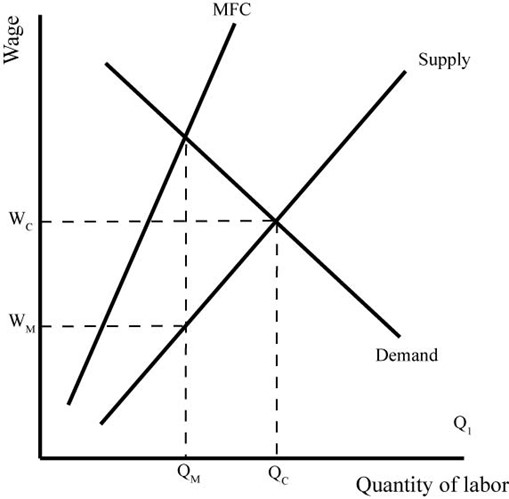
\includegraphics[width=0.5\textwidth]{images/monopsony.jpg}
    \end{solution}

\end{questions}

\end{document}